
\chapter*{\ding{167} \ding{167} \ding{167}}

\section*{Closing words on chapter 2}
Chapter 2 is a focused selection of terminology and concepts attained from the literature review that have been conducted throughout/during the thesis project. It is structured in the hoping that designers who is interested in the topic can adopt the concepts as a vocabulary and means for understanding some of what goes on in the museum world. To "talk the talk" and "walk the walk", dissect domain events and experiences,or  "get into the nitty-gritty". The literature review has nonetheless been crucial for the thesis evolution. On the one hand, it has influenced the research framing and interest, shaped and refined the research question, and leveraged the vocabulary when documenting/ recounting an exhibition- and installation experience. While on the other hand, it has influenced the convergent and divergent thought-process when going in-and-out/back-and-forth of practical and theoretical work, the designer role and the researcher role.

% The next three chapters differs from chapter 2 because of their direct and practical application. Shaping the rest of the thesis and used for critiquing of the exhibitions/ installations.
The next three chapters is a continuation of the literature review. Where Chapter 2 indirectly affect the thesis evolution, Chapter 3, 4 and 5 present three theoretical frameworks that have practically/directly guided e.g. data-gathering guides during fieldwork, both for observations, interviews and analytical critique. In addition to this, in chapter 6, we build upon and borrow concepts in the making of an analytical tool, my proposal as a new way of designing for meaningfulness.

\begin{itemize}
    \item Chapter 3: Hybrid place
    \item Chapter 4: Place as a dialogue
    \item Chapter 5: Sense-making
    \item Chapter 6: A new way to design for meaningfulness?
\end{itemize}
\par


\section*{Theory as an analytical tool}
In my attempt to answer how one can design meaningful interactive experiences in a museum space that addresses sustainability, I have chosen to look into three theoretical frameworks that give the means to understand interactive artefacts dialogic qualities - as an answer to how museum spaces can look at their respective installations and judge whether or not they stimulate the visitor to dialogue (conversations). The hypothesis is that there lies value for the museum to judge whether or not their installations promote dialogue. 

The use of theory is essential to any academic discipline. Before we embark on to the Theory chapters, it is necessary to go into how theory have been put to use throughout the thesis project. 

\begin{figure}[H]
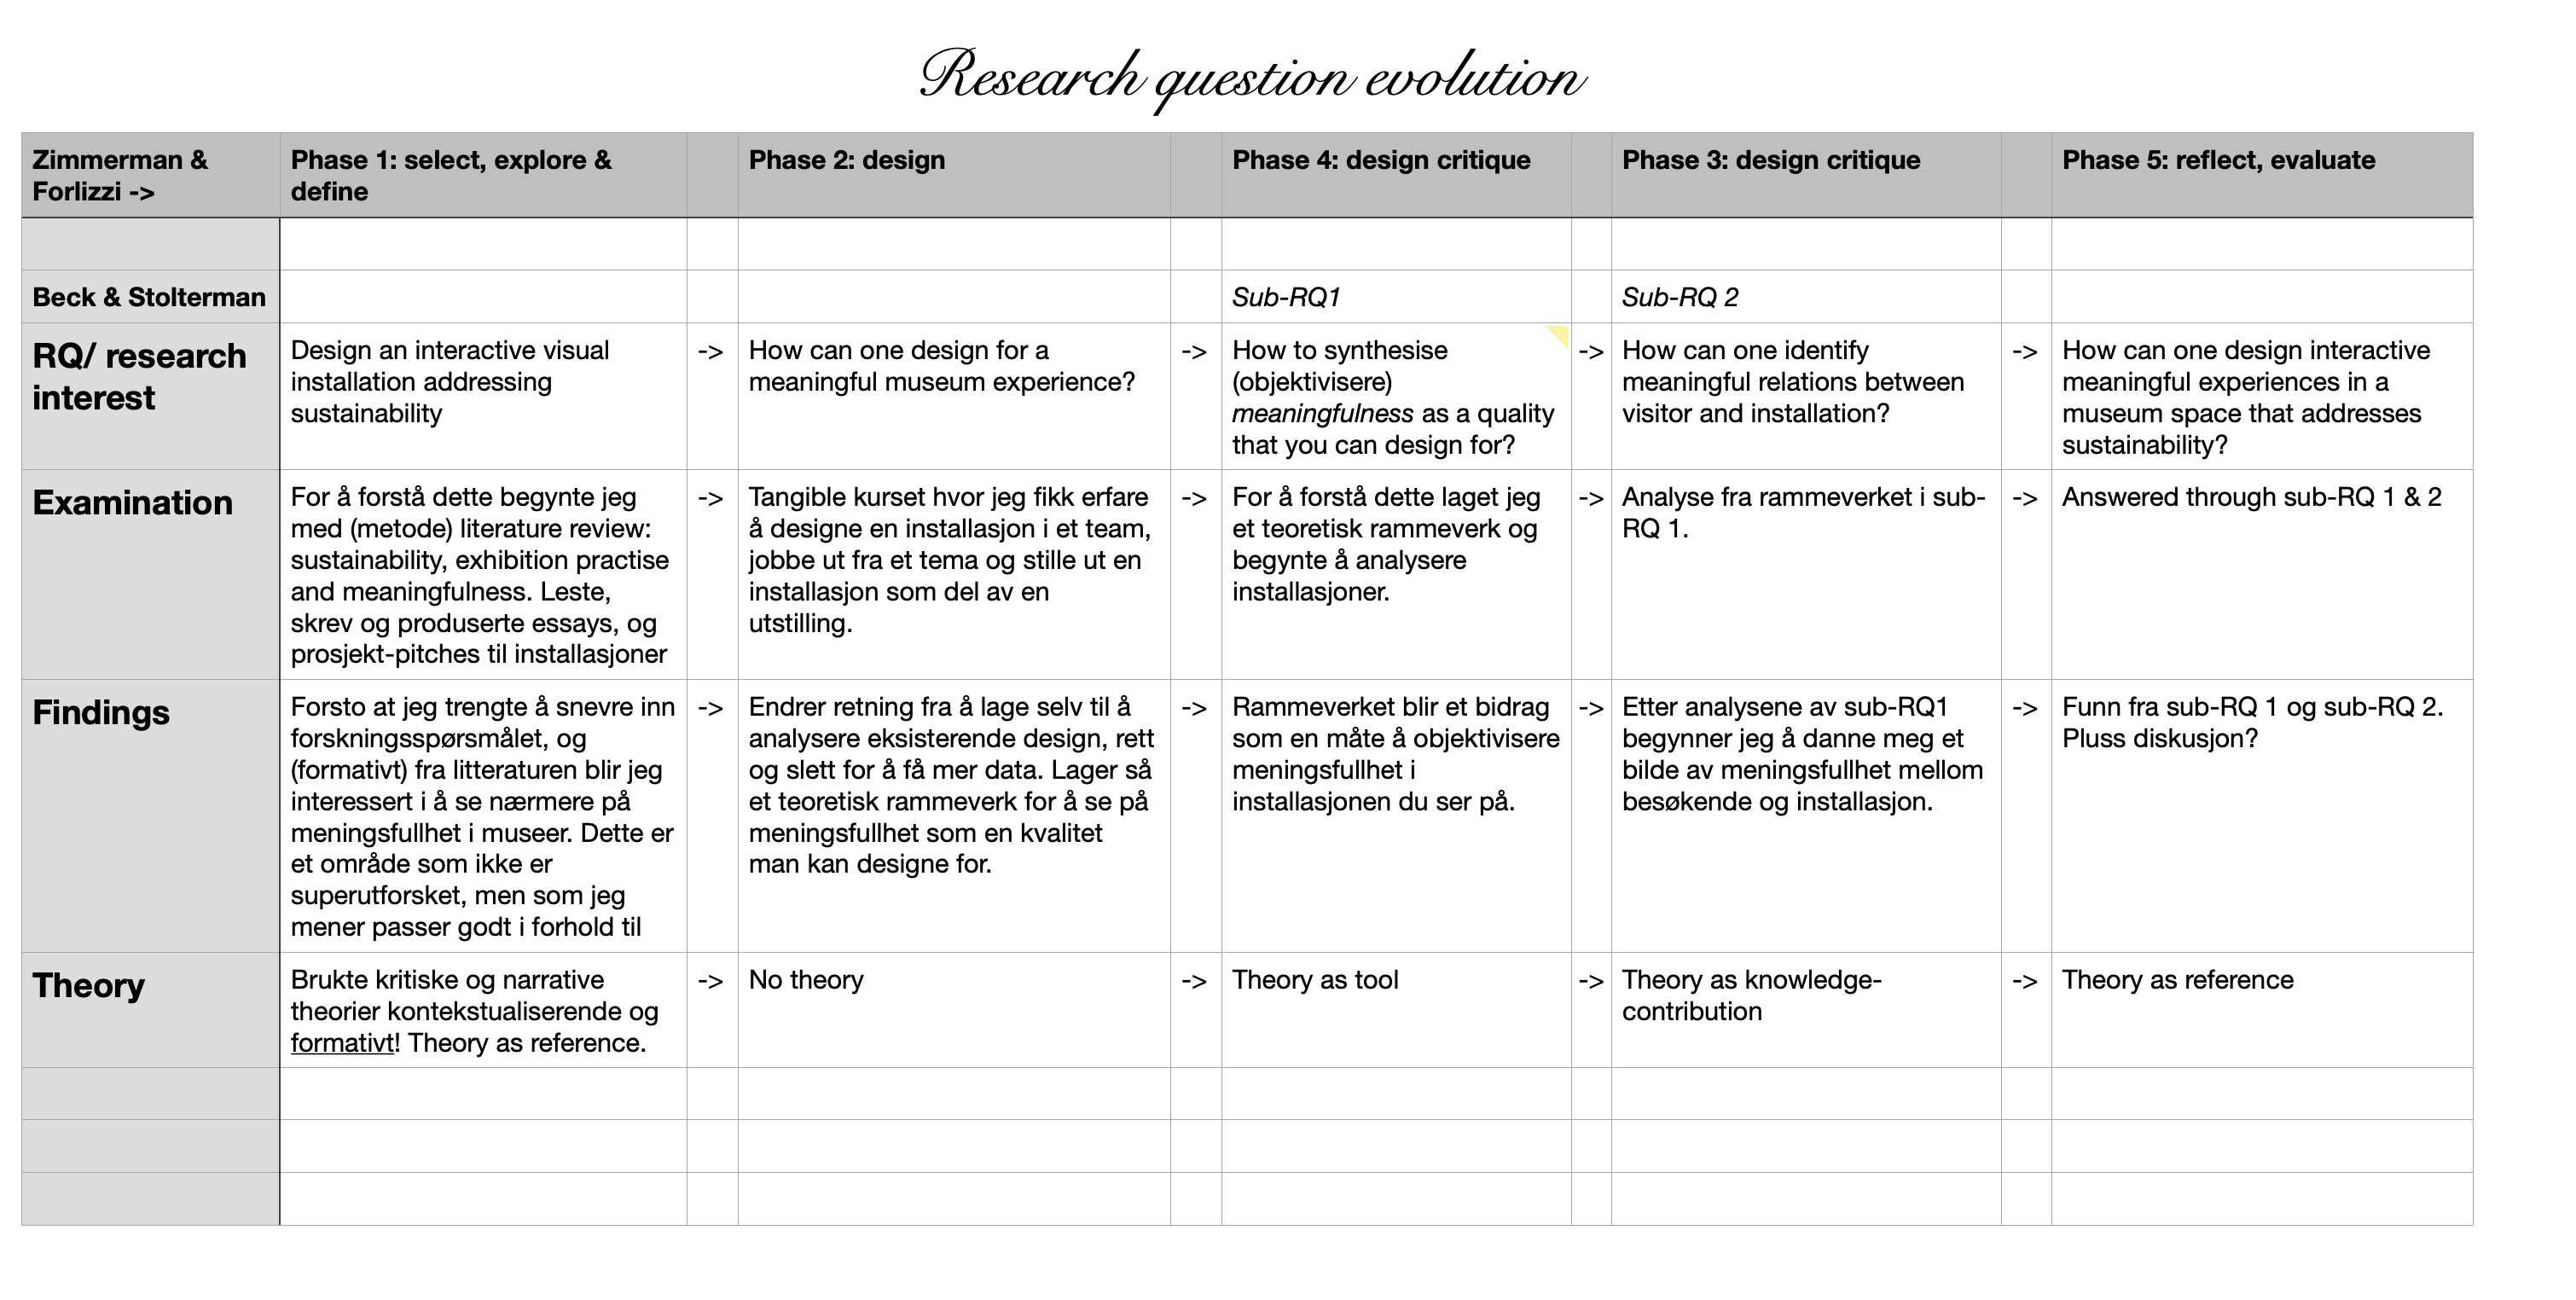
\includegraphics[width=21cm, angle=90]{pictures/process/rq_evolution.png}
\caption{Research question evolution}
\centering 
\end{figure}
